\documentclass[tikz,border=10pt]{standalone}

\usepackage{tikz}

\begin{document}

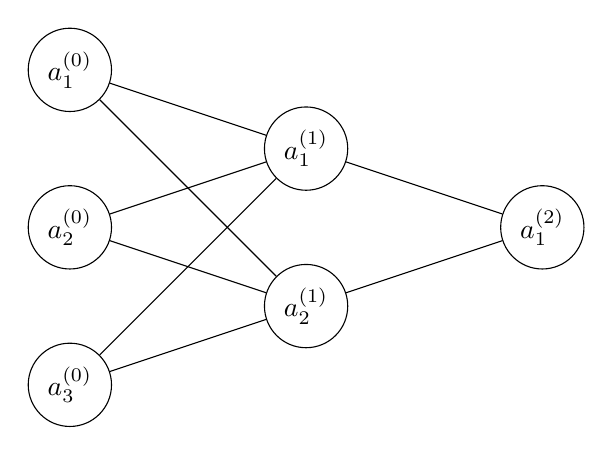
\begin{tikzpicture}[
    neuron/.style={circle, draw, minimum size=1cm}
]

    \node[neuron] (I1) at (0,6) {$a^{(0)}_1$};
    \node[neuron] (I2) at (0,4) {$a^{(0)}_2$};
    \node[neuron] (I3) at (0,2) {$a^{(0)}_3$};

    \node[neuron] (H1) at (3,5) {$a^{(1)}_1$};
    \node[neuron] (H2) at (3,3) {$a^{(1)}_2$};

    \node[neuron] (O1) at (6,4) {$a^{(2)}_1$};

    \draw (I1) -- (H1);
    \draw (I1) -- (H2);

    \draw (I2) -- (H1);
    \draw (I2) -- (H2);

    \draw (I3) -- (H1);
    \draw (I3) -- (H2);

    \draw (H1) -- (O1);
    \draw (H2) -- (O1);

\end{tikzpicture}

\end{document}
